%%%%%%%%%%%%%%%%%%%%%%%%%%%%%%%%%%%%%%%%%%%%%%%%%%%%%%%%%%%%%%%%%%%%%%%%%%%%%%%%
%%
%% Section: Overview
%%
%%%%%%%%%%%%%%%%%%%%%%%%%%%%%%%%%%%%%%%%%%%%%%%%%%%%%%%%%%%%%%%%%%%%%%%%%%%%%%%%
\section{Overview}

This tutorial will use the following definitions:

\begin{itemize}
\item
  \emph{data item} - this a basic unit of data of which you may have
  thousands and you wish to study the relationships these units. They
  may be proteins interacting with each other, or genes, or protein/DNA
  sequences, or \ldots{} --- you name it,
\item
  \emph{module} - a group of data items closely related to one another
  by some metric or property,
\item
  \emph{clustering} - a collection of modules, possibly overlapping.
\end{itemize}

\coral is a suite of visualizations that helps you compare multiple
clusterings at a time. For example, modules can constitute a collection
of genes that get co-expressed together or proteins forming a complex. A
\emph{clustering} usually is an output of a clustering algorithm. You
may also choose to group data according to attributes that come with the
data such as cellular component or molecular function GO terms and use
that partition as a clustering. You may combine data from different
experiments and across species so long as the data items that the user
treats as homologous have the same IDs across the dataset.

%%%%%%%%%%%%%%%%%%%%%%%%%%%%%%%%%%%%%%%%%%%%%%%%%%%%%%%%%%%%%%%%%%%%%%%%%%%%%%%%
%%
%% Section: running coral
%%
%%%%%%%%%%%%%%%%%%%%%%%%%%%%%%%%%%%%%%%%%%%%%%%%%%%%%%%%%%%%%%%%%%%%%%%%%%%%%%%%
\section{Running \coral}

\coral is a cross-platform desktop application written in Java. Start by 
downloading the application for your system from 
\url{www.cbcb.umiacs.umd.edu/kingsford-group/coral}. You should put the file in
the directory of your choice and unzip it.

If you have downloaded \coral package for MacOS, you should double click on 
\coral's icon in the folder you've just downloaded. This will launch the 
application with allocating 1Gb of memory for Java's heap.

You can run \coral from a command line by issuing the following command in the 
top-level \coral directory:
%
\begin{verbatim}
      $ ./coral
\end{verbatim}
%
in \coral's directory. This will run a shell script that launches \coral, and
tells Java to use 1Gb of memory for heap space. You can edit the script to 
allocate more memory for the heap which usually a good idea in case you have 
large clusterings or many of them. 




%%%%%%%%%%%%%%%%%%%%%%%%%%%%%%%%%%%%%%%%%%%%%%%%%%%%%%%%%%%%%%%%%%%%%%%%%%%%%%%%
%%
%% Section: Input
%%
%%%%%%%%%%%%%%%%%%%%%%%%%%%%%%%%%%%%%%%%%%%%%%%%%%%%%%%%%%%%%%%%%%%%%%%%%%%%%%%%
\section{Loading data}

The input files for \coral should each describe a single clustering with every 
line in the file corresponding to a single module. \coral expects the first item
on the line to be a module identifier, i.e.:
%
\begin{verbatim}
      1 AT3G13710 AT1G74520 AT1G17080 ...
      2 AT3G10340 AT3G53260 AT3G59940 ...
      3 AT1G70700 AT2G01570 AT1G53510 ...
     ...
\end{verbatim}
%
Here, 1, 2, and 3 are module identifiers followed by the protein IDs that form
those modules. Module names within a single clustering file have to be unique; 
if a module ID is repeated within a file, \coral reports a parsing error. \coral
assumes that each module should have an ID and at least one item in it; if a 
line describing a module only contains a module name or a single data item, 
\coral reports a parsing error. If the module name is omitted, and the line 
starts with data items in the module, the first data item would be parsed as the 
module name and will not be included as part of the module.

Users can use any latin and punctuation characters for their module and item 
names. Spaces and tabs can not be part of the name since they are reserved as 
separator characters. If you use spaces in your data item names, each part would
be parsed as a separate data item.

\begin{comment}
\begin{figure}[ht!]
  \centering
  \includegraphics[width=0.35\linewidth]{load_clusts}
  \caption{Loading data into \coral.}
  \label{fig:load}
\end{figure}
\end{comment}

Users can load the clustering files using a \texttt{File -> Open clusterings} 
menu option.%(Figure~\ref{fig:load}).


%%%%%%%%%%%%%%%%%%%%%%%%%%%%%%%%%%%%%%%%%%%%%%%%%%%%%%%%%%%%%%%%%%%%%%%%%%%%%%%%
%%
%% Section: Visualizations
%%
%%%%%%%%%%%%%%%%%%%%%%%%%%%%%%%%%%%%%%%%%%%%%%%%%%%%%%%%%%%%%%%%%%%%%%%%%%%%%%%%
\section{Using \coral views}

\coral consists of 6 linked views: selection in one view causes the application 
to select corresponding items in a different view making it easy to track groups
of items across the whole application.

\begin{figure}[ht]
  \centering
  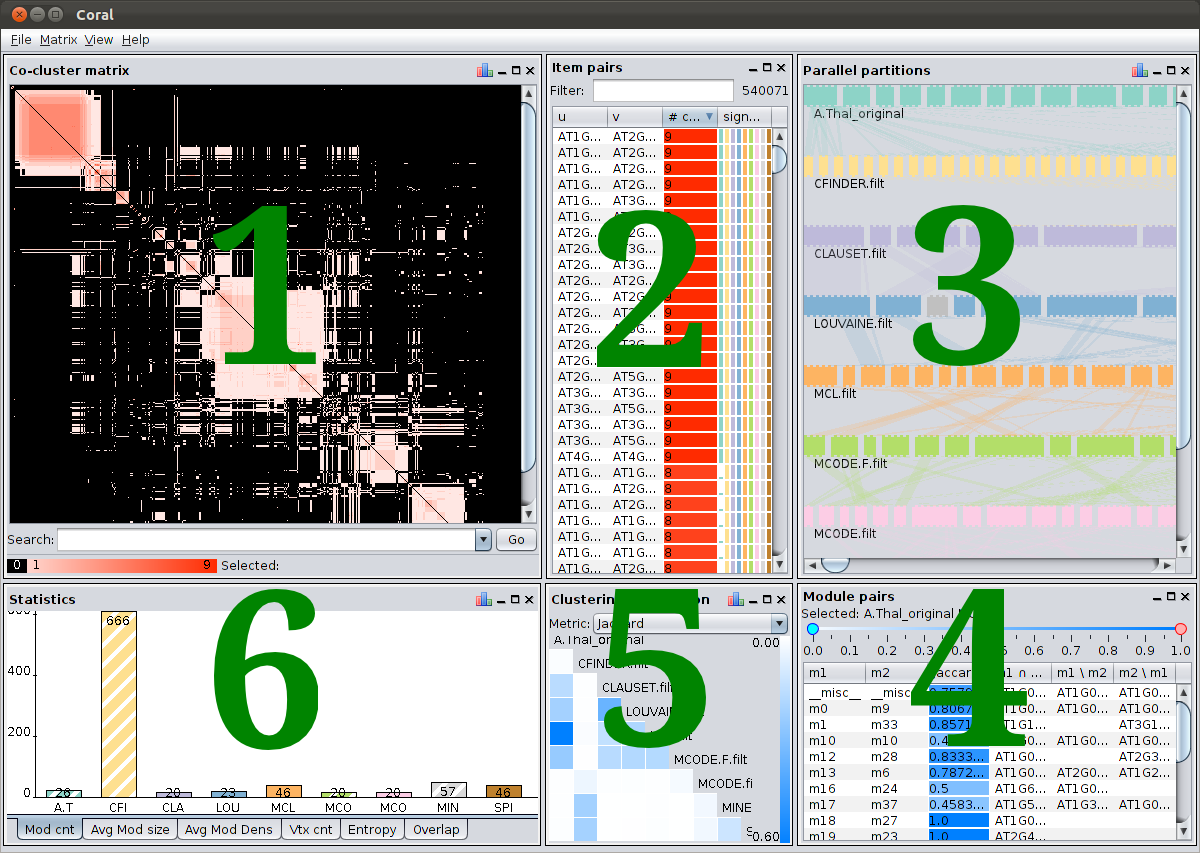
\includegraphics[width=\textwidth]{overview}
  \caption{\coral consists of 6 linked views: co-cluster matrix, item pairs 
    table, paralle partitions plot, modules table, comparison ladder, and 
    overview statistics.}
  \label{fig:overview}
\end{figure}


%%%%%%%%%%%%%%%%%%%%%%%%%%%%%%%%%%%%%%%%%%%%%%%%%%%%%%%%%%%%%%%%%%%%%%%%%%%%%%%%
\subsection{Co-cluster matrix}

In \coral, pairwise co-cluster memberships are aggregated in a 
\textit{co-cluster matrix}. Given a single clustering $K$, $n = |K|$, we define 
an $n \times n$ matrix $A^{K}$ to be $K$'s co-cluster matrix where its entries 
$a_{ij}^{K}$ are:
%
\[
 a_{ij}^{K} = 
  \begin{cases}
0 & \text{$v_{i}$ and $v_{j}$ are in different modules in $K$}\\
1 & \text{$v_{i}$ and $v_{j}$ are in the same module in $K$}.\\
  \end{cases}
\]
%
You can see a small example of two such co-cluster matrices for partitionings of
a small network in Figure~\ref{fig:co-clust-example}.
%
\begin{figure}[ht]
  \centering
  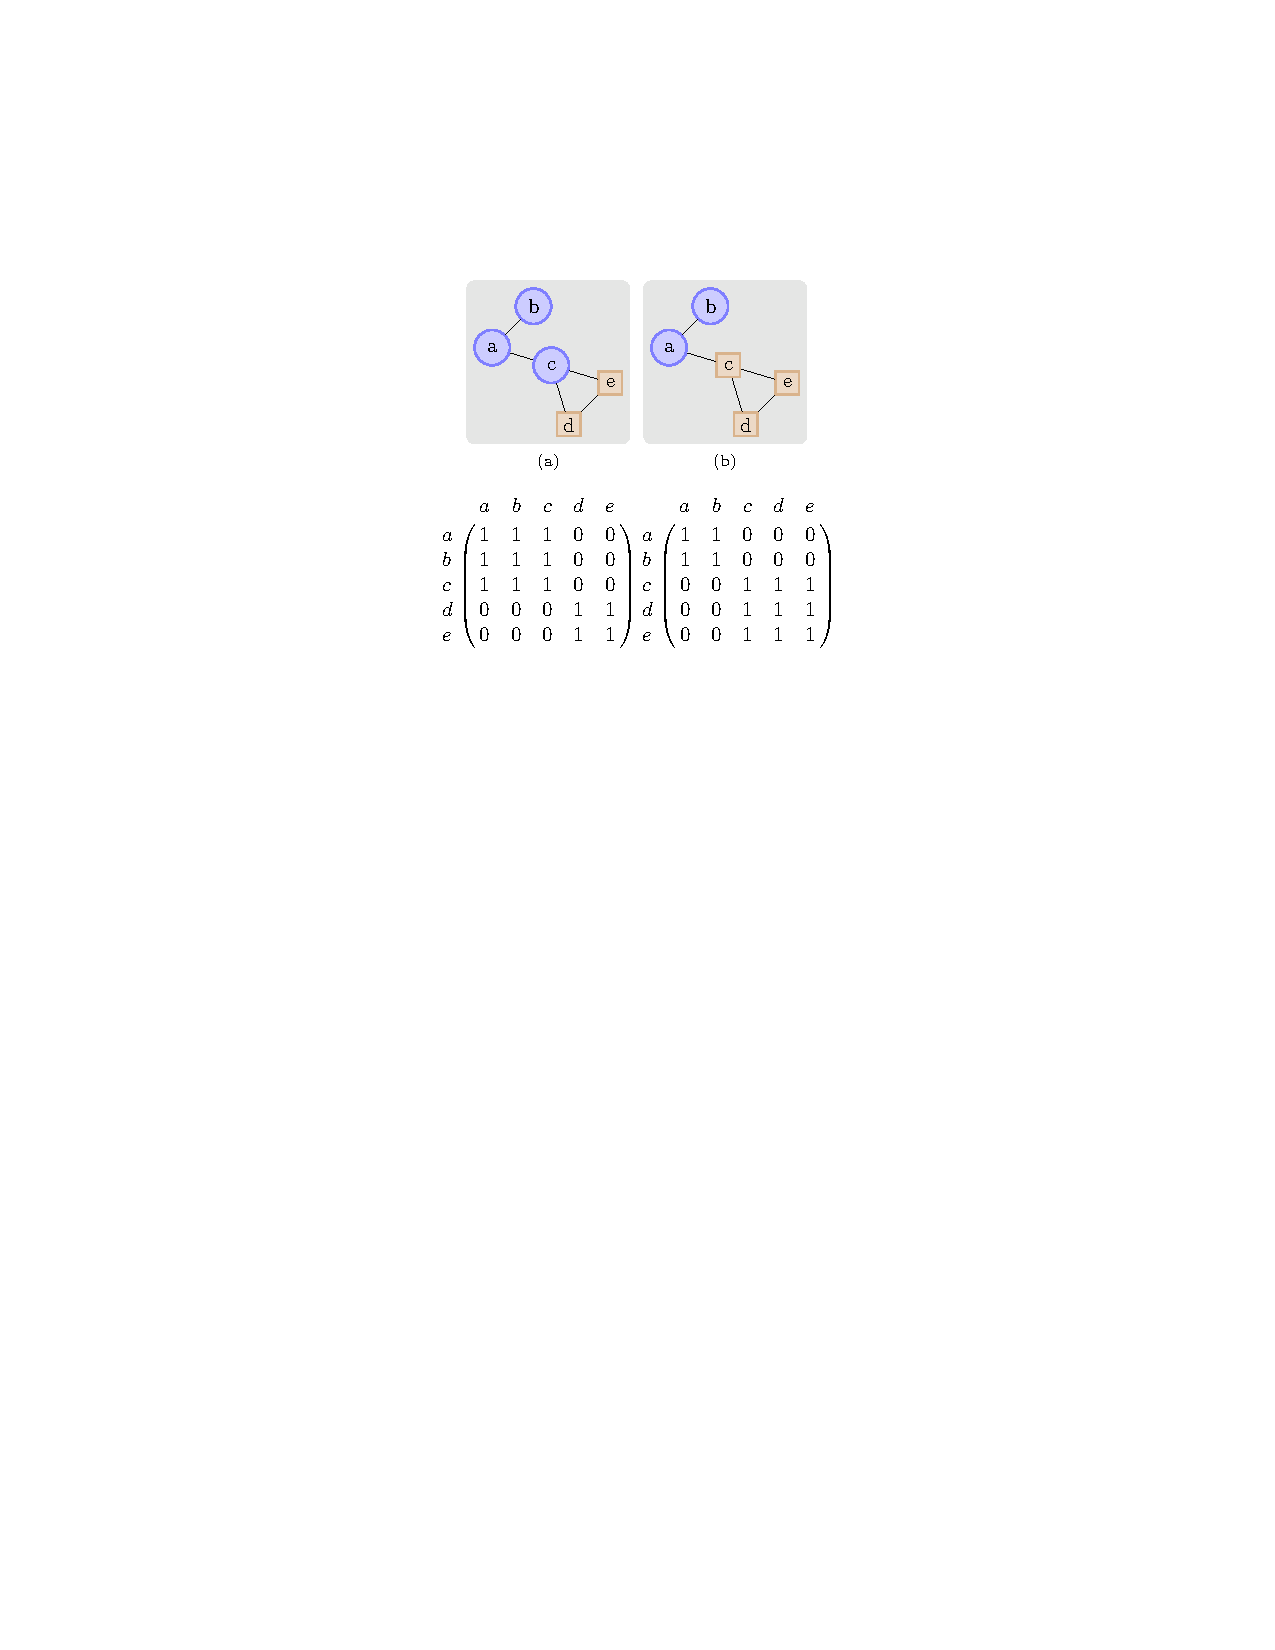
\includegraphics[width=0.5\textwidth]{co-clust-example}
  \caption{An example of two different clusterings of a small network and their
  corresponding co-cluster matrices. Blue and brown nodes represent two modules
  in the partitioning.}
  \label{fig:co-clust-example}
\end{figure}
%

We sum up the co-cluster matrices from individual clustering to form a single 
matrix:
%
\[
 A^{+} = \sum_{t=1}^{k} A^{K_{t}},
\]
%
where $A^{K_{t}}$ is a co-cluster matrix for a clustering $K_{t}$, and $k$ is the
number of clusterings. Here, the $a_{ij}^{+}$ entries equal $k$ (the number of 
clusterings) for item pairs $(v_{i}, v_{j})$ that have co-clustered in all 
partitions suggesting a strong relationship between the items, and the low 
$a_{ij}^{+}$ values correspond to pairs that co-clustered in only a few 
clusterings and are more likely to have been assigned to the same module by 
chance (see Figure~\ref{fig:co-clust}). The cells are colored according to their
values and vary from pale pink (low values) to red (high values).

You can zoom in and out on sections of the matrix with a scroll wheel. When 
matrix does not fit on the screen, the scrollbars appear, and you can recenter 
the matrix on the region of interest.

If the clusterings are identical, the co-cluster matrix would look like 
Figure~\ref{fig:identical-clust}. A single clustering with overlapping modules
would produce a matrix like in Figure~\ref{fig:overlapping-clust}. Clusterings
that have a high amount of disagreement may look like Figure~\ref{fig:disagreeing-clust}.


\begin{figure}[ht]
  \centering
  \begin{subfigure}[b]{0.1\textwidth}
    \centering
    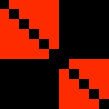
\includegraphics[width=\textwidth]{identical-clust}
    \caption{}
    \label{fig:identical-clust}
  \end{subfigure}
  %
  \begin{subfigure}[b]{0.1\textwidth}
    \centering
    
\includegraphics[width=\textwidth]{overlapping-clust}
    \caption{}
    \label{fig:overlapping-clust}
  \end{subfigure}
  %
  \begin{subfigure}[b]{0.1\textwidth}
    \centering
    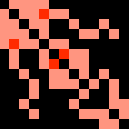
\includegraphics[width=\textwidth]{disagreeing-clust}
    \caption{}
    \label{fig:disagreeing-clust}
  \end{subfigure}

  \caption{Various co-cluster matrices. (a) Several identical non-overlapping 
    clusterings. (b) A single clustering with overlapping modules. (c) Two 
    disagreeing non-overlapping clusterings.}
  \label{fig:co-clust}

\end{figure}

\subsubsection{Reordering matrix}

The amount of information you can learn from the matrix depends on the order of
its rows and columns. \coral uses a SPIN algorithm~\cite{SPIN} for finding an 
ordering of rows and columns that pushes non-zero matrix elements towards the 
matrix diagonal. Greedy vs optimal. Iterations. More interations - better 
solution, but longer time.

To reorder your matrix, you can navigate to \texttt{Menu->Matrix->Reorder}. 
You will see a dialog box asking you to specify how many times to apply one of 
the reordering techniques. You can set the counter to 0 if you do not want that
reordering technique to run at all.

\begin{figure}
  \centering
  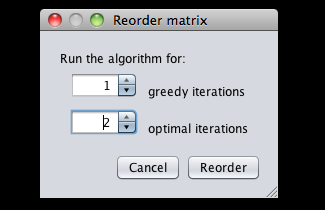
\includegraphics[width=0.45\linewidth]{reorder-diag}
  \caption{TODO}
  \label{fig:reorder-diag}
\end{figure}


\subsubsection{Selecting a base matrix}


%%%%%%%%%%%%%%%%%%%%%%%%%%%%%%%%%%%%%%%%%%%%%%%%%%%%%%%%%%%%%%%%%%%%%%%%%%%%%%%%
\subsection{Item pairs table}

\newcommand{\Athal}{\textit{A. thaliana}}

An item pairs table facilitates sorting and search for particular item pairs 
that have co-clustered together at least once. In other words, every non-zero 
element in the co-cluster matrix gets a row in the pairs table. Each row in the 
table represents a pair of data items and displays the number of times the items 
co-clustered along with the pair's \textit{signature}. The signature is a 
$k$-long vector where the $t^{th}$ element is 1 when both data items, say, 
proteins, have been placed in the same module in clustering $K_{t}$. If the 
pair's items were not in the same module in $K_{t}$, the $t^{th}$ element is set
to 0.

Visually, the signature's elements that are 1 are drawn as tall
solid columns and zeros are represented by the short stumps using the same color
for each clustering as is used in the overview statistics 
(Subsection~\ref{sec:stats}) and in the parallel partitions plot. 
Figure~\ref{fig:signature} shows an example of two such pairs that have 
different co-cluster signatures suggesting that the relationship between the 
last two \Athal proteins is stronger than that of the first pair. Users can sort
the rows by either the item name, the number of shared clusterings, or by the 
co-clustering signature. Users can also filter by the signatures to display only
the rows matching a user's pattern.

\begin{figure}[ht]
	\centering
    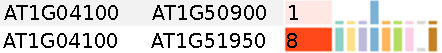
\includegraphics[width=0.3\linewidth]{item-pair-crisp.pdf}
	\caption{TODO}
	\label{fig:signature}
\end{figure}

You can filter the table based on the signatures by defining a regular 
expression in the textbox above the table (Figure~\ref{fig:filter-pairs}) and 
hitting the "Enter" key. Only rows that match the provided pattern would remain 
in the table. The row count (to the right of the pattern textbox in 
Figure~\ref{fig:filter-pairs}) would reflect the number of rows that matched.
Here are the rules for writing a pattern: if you want the signature to have a 1 
in position $t$, then put a 1 in the pattern at that position. If you want 
$t^{th}$ element to be 0, then substitute 1 for a 0. If you do not care whether 
it is a 1 or a 0, then put a dot (.) in the position. In addition, you do not 
have to specify all $k$ elements, only the first few you are interested in. In 
the example below, the pattern "1.1111" means that I want to see all pairs of 
data items that have co-clustered together in clusterings 1, 3, 4 and 5, but it 
does not matter if data items have been placed together in clustering 2. 
Omitting the last digits in hte pattern is equivalent to writing "1.1111....", 
i.e. it is saying that it does not matter whether data items have co-clustered 
in the last four clusterings. The results reflect this:
%
\begin{figure}[ht]
  \centering
  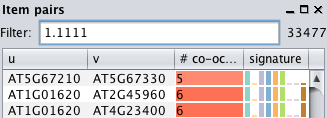
\includegraphics[width=0.39\textwidth]{filter-pairs}
  \caption{TODO}
  \label{fig:filter-pairs}
\end{figure}
%
The first and second pairs' signatures show two ways to match the pattern. 
By scrolling futher down the table, we see more rows that matched for a total of
33477 rows with this pattern. For the same dataset, replacing a dot in the 
second position (111111) reduces the number of matched rows to 299, and only 21
rows match the pattern of all ones for each clustering --- only 21 item pairs
have co-clustered in all of the clusterings in the dataset.


%%%%%%%%%%%%%%%%%%%%%%%%%%%%%%%%%%%%%%%%%%%%%%%%%%%%%%%%%%%%%%%%%%%%%%%%%%%%%%%%
\subsection{Parallel partitions}

\newcommand{\pthree}{$P^{3}$\xspace}

The parallel partitions plot (\pthree) represents each clustering as a horizontal band. 
The blocks comprising each bands represent modules, with the width of a block 
proportional to the number of items in that module. Semi-transparent 
parallelograms between clusterings connect data items with the same name. That 
is, each item in a clustering will be connected to its copy in the band 
immediately below it (see Figure ~\ref{fig:ppp}).

\begin{figure}
  \centering
  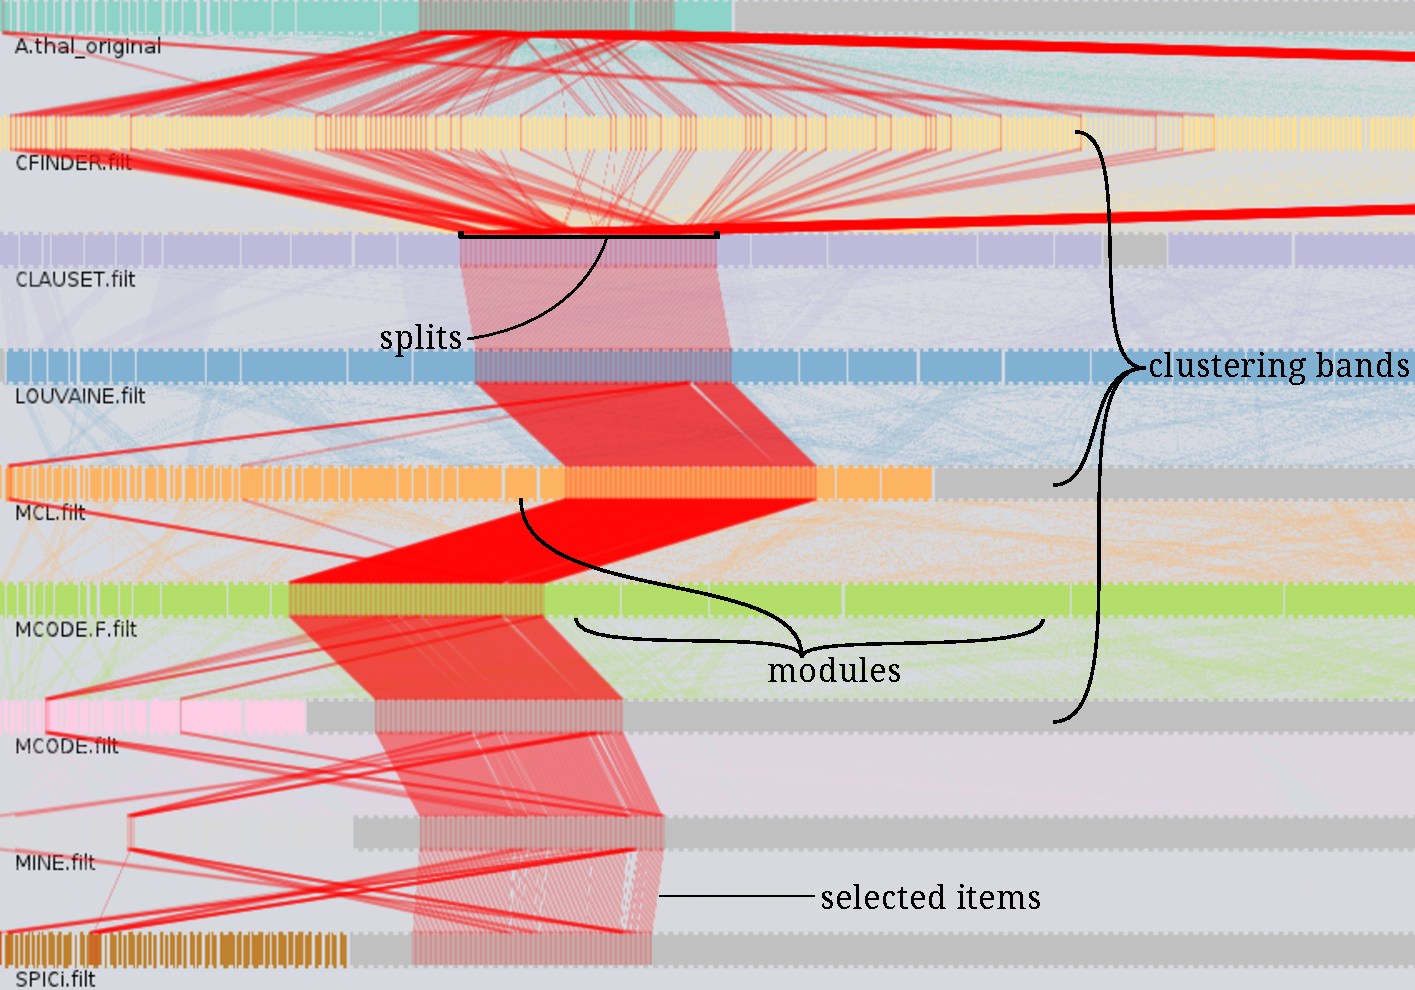
\includegraphics[width=0.8\textwidth]{ppp}
  \caption{}
  \label{fig:ppp}
\end{figure}

Users can select a module with a mouse while holding a "Shift" key to highlight 
its members in every clustering in the plot (see red traces in Figure~\ref{fig:ppp}). 
Similarly, users may select individual items and trace them through every 
clustering band. The selections made in the parallel partitions plot propagate 
to other views making it easy to track the same group of items throughout the 
application. The plot is zoomable — users may zoom in to focus on a few items at
a time or zoom out to see global trends across the ensemble. When the zoom level
permits it, the plot displays the item labels.

Gray bar in \pthree


%%%%%%%%%%%%%%%%%%%%%%%%%%%%%%%%%%%%%%%%%%%%%%%%%%%%%%%%%%%%%%%%%%%%%%%%%%%%%%%%
\subsection{Module-to-module table}

When users select a pair of clusterings using the ladder widget, the module 
table

%%%%%%%%%%%%%%%%%%%%%%%%%%%%%%%%%%%%%%%%%%%%%%%%%%%%%%%%%%%%%%%%%%%%%%%%%%%%%%%%
\subsection{Ladder widget}


The ladder widget represents a lower triangle of an all-to-all comparison 
matrix between every pair of clusterings. For example, in 
Figure~\ref{fig:ladder}, the ladder shows Jaccard similarity between ten 
different clusterings of a small social network. Cells are color-coded with more
intense blue cells corresponding to pairs of clusterings of higher similarity.
Users may choose between several similarity metrics discussed in 
Section~\ref{sec:sim_metr}.


\begin{comment}
\[
 \begin{array}{c|c|c}
  s(1,2) &  &  \\
  \hline
  s(1,3) & s(2,3) & \\
  \hline
  s(1,4) & s(2,4) & s(3,4)  \\
 \end{array}
\]
\end{comment}

\begin{figure}
  \centering
  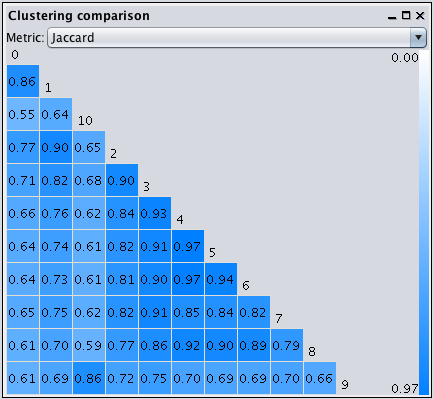
\includegraphics[width=0.3\linewidth]{ladder.png}
  \caption{}
  \label{fig:ladder}
\end{figure}

TODO: clicking


%%%%%%%%%%%%%%%%%%%%%%%%%%%%%%%%%%%%%%%%%%%%%%%%%%%%%%%%%%%%%%%%%%%%%%%%%%%%%%%%
\subsection{Overview statistics}
\label{sec:stats}

Overview statistics are rendered as bar charts with each bar corresponding to 
the value of a statistics of a single clustering. If a clustering contains 
overlapping modules, some of the statistics (such as the average module size or
entropy) may be skewed -- the bars for such clusterings are drawn using a hashed
pattern (see Figure~\ref{fig:overview}, area 6: the tall yellow bar represents 
one such clustering).

\textbf{Module count} --- shows the number of modules in each clustering. The
\grabbag module is not included in this count.

\textbf{Average module size} --- shows the average module size per clustering. 
Computed as $ \sum_{i} m_{i}  / m $ where the numerator represents the sum of 
aizes across all modules (excluding the \grabbag) and the denominator represents
the number of modules considered in the numerator.

\textbf{Average module density} --- XXX (e/v or e/chose2). Only available for the network modules and 
requires that the original network is loaded.

\textbf{Item count*} --- displays the total number of data items that were 
assigned to some module by the given clustering. * in older versions of \coral
``item count'' was called ``vertex count''.

\textbf{Entropy} --- displays the entropy value for each clustering giving an 
idea of how skewed the distribution of module sizes is. Entropy of a clustering
$K$ is computed as $-\sum_{m \in K} p_{m} \log_{2} p_{m}$ where 
$p_{m} = |m| / |K|$ is a probability of a data item being assigned to module $m$.

\textbf{Overlap} --- displays the percentage of data items included in the 
clustering that were assigned to more than one module.


%%%%%%%%%%%%%%%%%%%%%%%%%%%%%%%%%%%%%%%%%%%%%%%%%%%%%%%%%%%%%%%%%%%%%%%%%%%%%%%%
%%
%% Section: Overview
%%
%%%%%%%%%%%%%%%%%%%%%%%%%%%%%%%%%%%%%%%%%%%%%%%%%%%%%%%%%%%%%%%%%%%%%%%%%%%%%%%%
\section{Similarity metrics}
\label{sec:sim_metr}

The ladder widget offers users a choice of several metrics for evaluating 
similarity between pairs $K_{i}, K_{j}$ of clusterings within an ensemble. The 
first four measures are based on the pair counting; the next two are based on
information theory; the last 3 measures are based on set matching.

There are four quantities on which pair counting measures are based:

  $a$ -- number of item pairs placed in a module together in clustering $K_{i}$ 
    as well as in clustering $K_{j}$,

  $b$ -- number of item pairs placed in a module together in clustering $K_{i}$,
    but not in clustering $K_{j}$,

  $c$ -- number of item pairs placed in separate modules in $K_{i}$, but in the 
    same module in $K_{j}$,

  $d$ -- number of item pairs placed in separate modules in both $K_{i}$ and 
    $K_{j}$.

%
\begin{description}
  \item[Jaccard] \hfill \\
  $a / (a + b+ c)$,

  \item[Mirkin] \hfill \\
  blah
  \item[Rand] \hfill \\
  The third etc \ldots
  \item[Folkes-Mallows] \hfill \\
  The third etc \ldots
  \item[Mututal information] \hfill \\
  The third etc \ldots
  \item[Variation of information] \hfill \\
  The third etc \ldots
  \item[Purity] \hfill \\
  The third etc \ldots
  \item[Inverse purity] \hfill \\
  The third etc \ldots
  \item[F-measure] \hfill \\
  The third etc \ldots
\end{description}
%



%%%%%%%%%%%%%%%%%%%%%%%%%%%%%%%%%%%%%%%%%%%%%%%%%%%%%%%%%%%%%%%%%%%%%%%%%%%%%%%%
%%
%% Section: running coral
%%
%%%%%%%%%%%%%%%%%%%%%%%%%%%%%%%%%%%%%%%%%%%%%%%%%%%%%%%%%%%%%%%%%%%%%%%%%%%%%%%%
\section{Managing windows}



%%%%%%%%%%%%%%%%%%%%%%%%%%%%%%%%%%%%%%%%%%%%%%%%%%%%%%%%%%%%%%%%%%%%%%%%%%%%%%%%
%%
%% Section: Overview
%%
%%%%%%%%%%%%%%%%%%%%%%%%%%%%%%%%%%%%%%%%%%%%%%%%%%%%%%%%%%%%%%%%%%%%%%%%%%%%%%%%
\section{Clustering algorithms}



%%%%%%%%%%%%%%%%%%%%%%%%%%%%%%%%%%%%%%%%%%%%%%%%%%%%%%%%%%%%%%%%%%%%%%%%%%%%%%%%
%%
%% Section: Overview
%%
%%%%%%%%%%%%%%%%%%%%%%%%%%%%%%%%%%%%%%%%%%%%%%%%%%%%%%%%%%%%%%%%%%%%%%%%%%%%%%%%
\section{Errors and exceptions}


%%%%%%%%%%%%%%%%%%%%%%%%%%%%%%%%%%%%%%%%%%%%%%%%%%%%%%%%%%%%%%%%%%%%%%%%%%%%%%%%
%%
%% Section: symbols and abbreviations used
%%
%%%%%%%%%%%%%%%%%%%%%%%%%%%%%%%%%%%%%%%%%%%%%%%%%%%%%%%%%%%%%%%%%%%%%%%%%%%%%%%%
\section{Symbols}

$K$ -- a single clustering,

$m_{i}^{j}$ -- an $i^{th}$ module in a clustering $j$,

$n = |K|$ -- number of data items considered in the clustering $K$,

$A^{K}$ -- co-cluster matrix for a single clustering $K$,

$a_{ij}^{K}$ -- an element of a co-cluster matrix for a clustering $K$, a 0 or a 1,

$A^{+}$ -- a sum of co-cluster matrices for a collection of $k$ clusterings 
  $K_{1}, \ldots, K_{k}$,

$a_{ij}^{+}$ -- an element of a co-cluster matrix, ranges from 0 to $k$,

$k$ -- number of clusterings in an ensemble,

$E_{\textrm{in}}$ -- the number of edges with both endpoints within a given 
  module

$E_{\textrm{out}}$ -- the number of edges with only a single endpoint within a 
  given module


